\documentclass[12pt,a4paper]{article}

\usepackage[margin=1in]{geometry}
\usepackage{fancyhdr}
\usepackage{graphicx}
\usepackage{epsfig}
\usepackage{parskip}
\usepackage[ansinew]{inputenc}
\usepackage{amsmath}
\usepackage{amssymb}
\usepackage{bm}
\usepackage{float}
\usepackage[free-standing-units=true]{siunitx} % for consistent handling of SI units
\usepackage[colorlinks=true, pdfstartview=FitV, linkcolor=blue, citecolor=blue, urlcolor=blue]{hyperref} % enable links

\setlength{\parindent}{0pt}

\newcommand{\m}[1]
{\mathrm{#1}}

\title{Experiment 9: Absolute Zero}
\author{Noa Sendlhofer, Christian Leser}
\date{\today}

\begin{document}

\maketitle

\begin{abstract}
    The goal of this experiment series is to determine the temperature of absolute zero, 
    as well as the temperature of liquid nitrogen. An apparatus of constant volume is filled with a gas
    and connected to a pressure sensor. Changing temperatures result in changes in pressure inside the chamber.
    Influences like the pressure and temperature inside the lab, as well as the expansion of the chamber itself
    in changing temperatures must be considered when discussing the obtained data. We concluded that the temperature
    of absolute zero $t_0 = (-275.9 \pm 2.45)\si{\bf\celsius}$ and the temperature of liquid nitrogen $t_{LN2} = (-198.5 \pm 2.56)\si{\bf\celsius}$.
    The literature values lie within our error margins.

\end{abstract}

\tableofcontents

\section{Introduction}

    % Interference double-silt source: https://wiki.anton-paar.com/ch-de/doppelspaltexperiment/
    % Interference grating source: https://www.grund-wissen.de/physik/optik/wellenoptik.html
    % Grating constant source: https://ieeexplore.ieee.org/stamp/stamp.jsp?tp=&arnumber=5547333&tag=1 (eth network)
    % Lands Pits CD source: https://www.researchgate.net/figure/Lands-and-pits-image-using-a-scanning-electron-microscope_fig3_221291847
    

    The goal of this experiment series is to build a spectrometer using household objects by making use of the wave character of light.
    To understand how the spectrometer works, we need to take a close look at how light behaves under certain conditions.

    \begin{figure}[H]
        \centering
        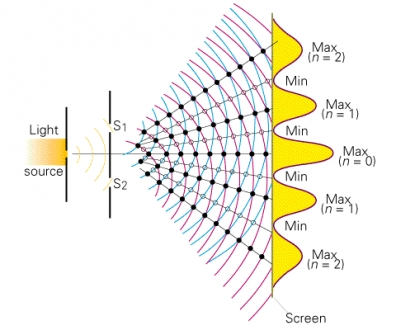
\includegraphics[scale = 0.7]{src/images/interference_double_slit.jpg}
        \caption{Double slit experiment.
        The interference of the light waves produce aspecific pattern which depends of the wavelength of the light entering the slits as well as the distance between the slits. \cite{src_double_slit}}
        \label{fig_double_slit}
    \end{figure}

    Light travels in a spherical way behind a slit meaning that each slit acts as a new source of waves.
    These waves interfere with each other as they overlap, resulting in an interference pattern of alternating bright and dark regions on the screen or detector.
    This behaviour is due to the fact that two maxima or minima intensify each other while a maximum and a minimum cancel out.
    We also refer to these two cases as constructive and destructive.
    Figure~\ref{fig_double_slit} shows how this effect works.

    \begin{minipage}{0.99\linewidth}
        \begin{minipage}{0.7\linewidth}
            \begin{figure}[H]
                \centering
                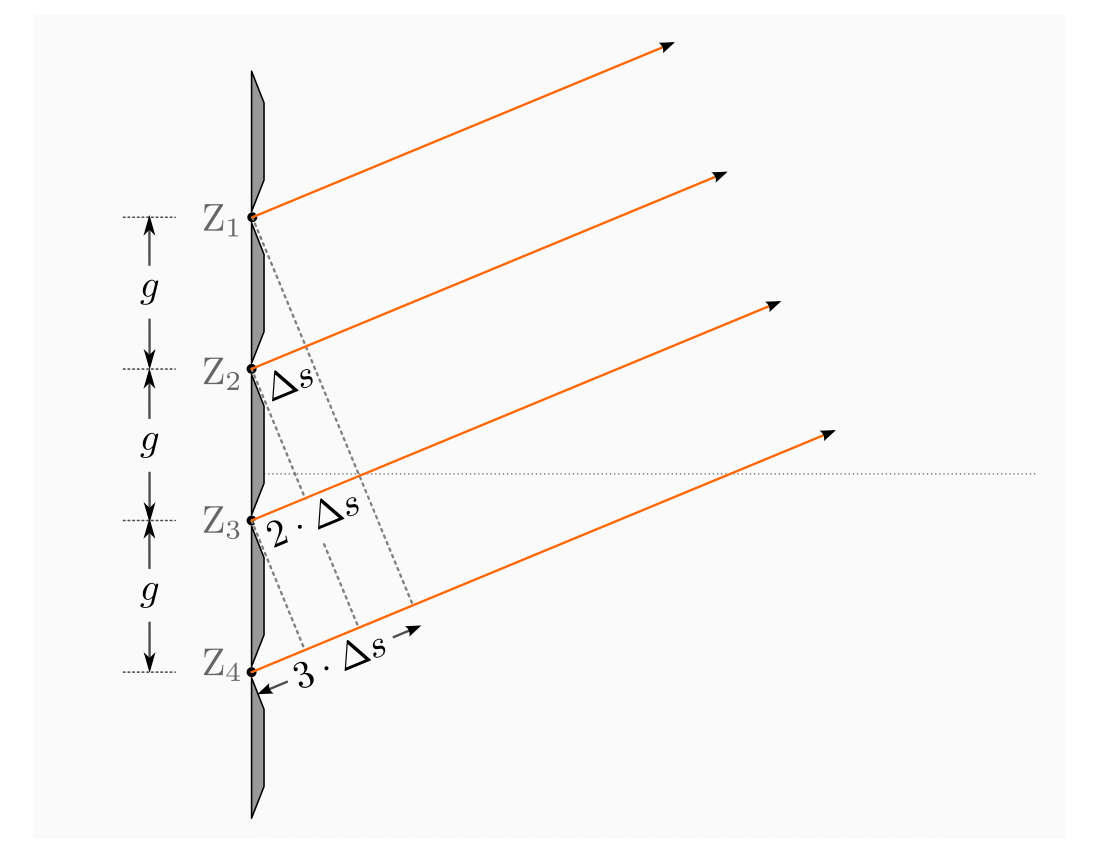
\includegraphics[scale = 0.25]{src/images/interference_grating.png}
                \caption{A grating leads to a similar effect as a double slit.
                $\Delta s$ is equal to the wavelength.
                As seen in the figure, the angle at which brighter spots of light can be seen depends on the wavelength. \cite{src_grating}}
                \label{fig_grating}
            \end{figure}
        \end{minipage}
        \begin{minipage}{0.25\linewidth}
          \begin{scriptsize}
            \begin{center}
                \begin{figure}[H]
                    \centering
                    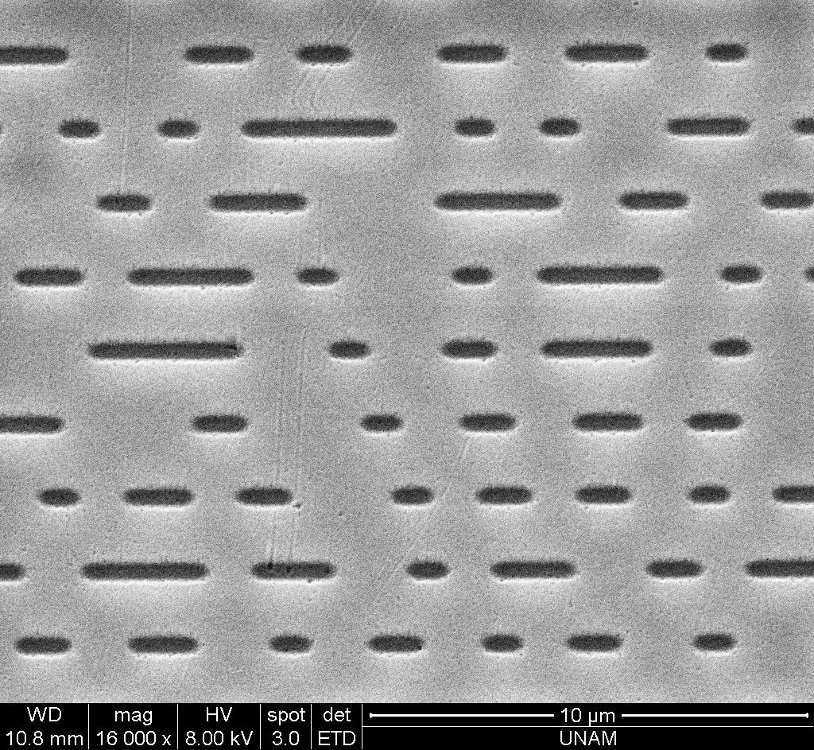
\includegraphics[scale = 0.15]{src/images/lands_pits_cd.png}
                    \caption{Lands and pits image of a CD using a scanning electron microscope. These form a grating too. \cite{src_cd}}
                    \label{fig_lands_pits}
                \end{figure}
            \end{center}
            \end{scriptsize}
        \end{minipage}
    \end{minipage}

    Moving on to a grating, it can be abstracted as a lot of slits next to each other.
    Hence, the effect is almost the same as the one observed at the double slit.
    Most importantly, an interference pattern can be observed too.
    When taking a close look at a CD, we notice a grating, presented in figure~\ref{fig_lands_pits}.
    In consequence, a CD must also produce an interference pattern in which light of different wavelength can be observed and distinguished.
    The characterisation of the light is done by measuring the distance of the maximum of first order as it is dependent of the wavelength.

    \begin{minipage}{0.99\linewidth}
        \begin{minipage}{0.45\linewidth}
            \begin{figure}[H]
                \centering
                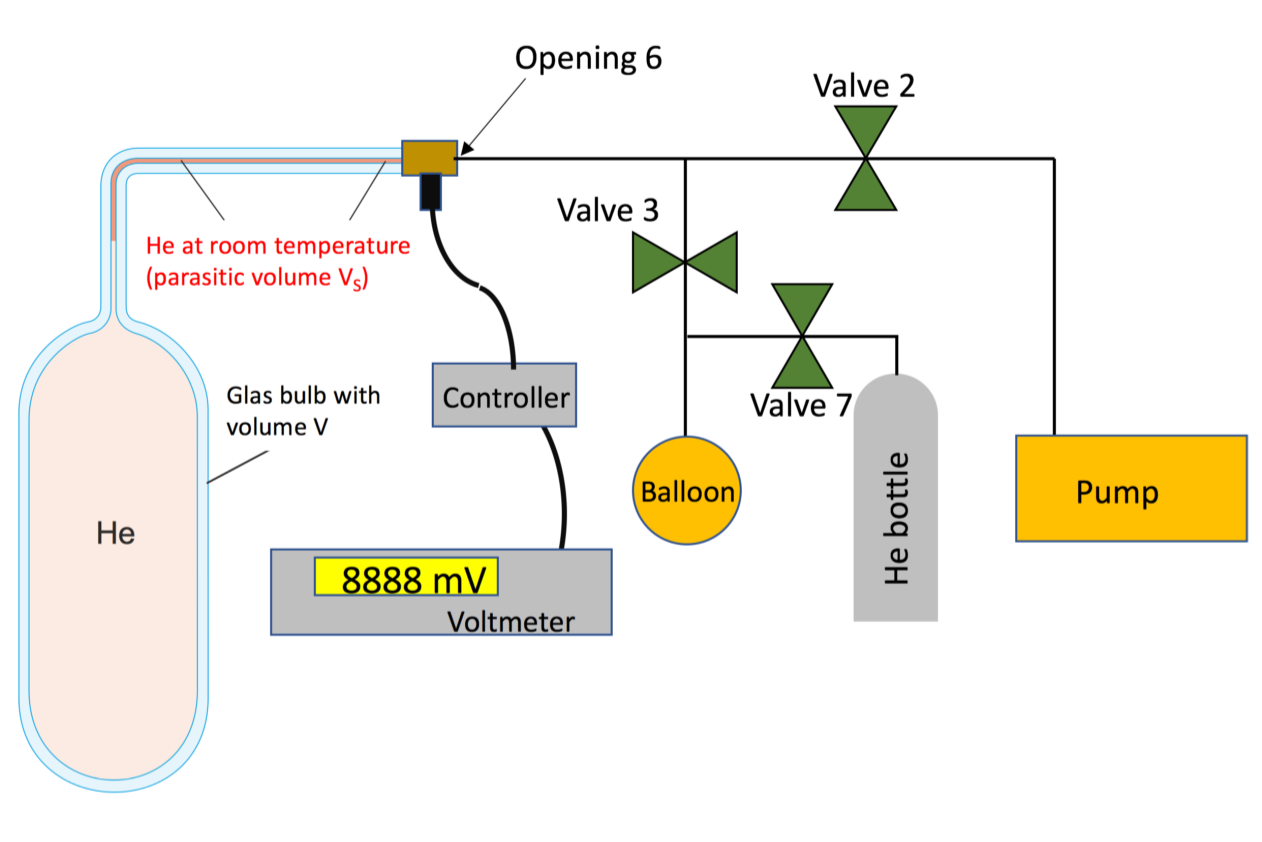
\includegraphics[scale = 0.4]{src/images/experimental_setup.png}
                \caption{Schematic of the experimental setup.
                A source emits rays of light of which a small portion enters the apparatus through a gap between two razor blades of about 0.2 mm.
                the light then travels through the dark chamber, until it hits the CD.
                After passing through the grid on the CD, an interference pattern can be detected using a camera.}
                \label{fig_setup}
            \end{figure}
        \end{minipage}
        \begin{minipage}{0.1\linewidth}
        \end{minipage}
        \begin{minipage}{0.45\linewidth}
          \begin{scriptsize}
            \begin{center}
                \begin{figure}[H]
                    \centering
                    \includegraphics[scale = 0.05]{src/images/spectrometer.png}
                    \caption{Experimental setup used in our case.
                    A phone is used as the camera to detect the interference pattern.}
                    \label{fig_spectrometer}
                \end{figure}
            \end{center}
            \end{scriptsize}
        \end{minipage}
      \end{minipage}
    


    % In general this section should tell the reader why he or she should
    % be interested in your paper. Give some background to the
    % experiment, and describe the underlying principles. This is typically where you provide references to previous publications~\cite{Sato2003}.

\section{Methods}
    We have multiple goals in this experiment series:
    \begin{enumerate}
        \item The calibration of the pressure sensor and its corresponding pressures.
        \item Determination of the absolute zero point of temperature.
        \item Determination of the temperature of liquid nitrogen.
    \end{enumerate}
    We will achieve these results by making use of the linearly corresponding properties of ideal gases with the help of the apparatus shown in Fig.~\ref{fig_setup}.

    \begin{figure}[H]
        \centering
        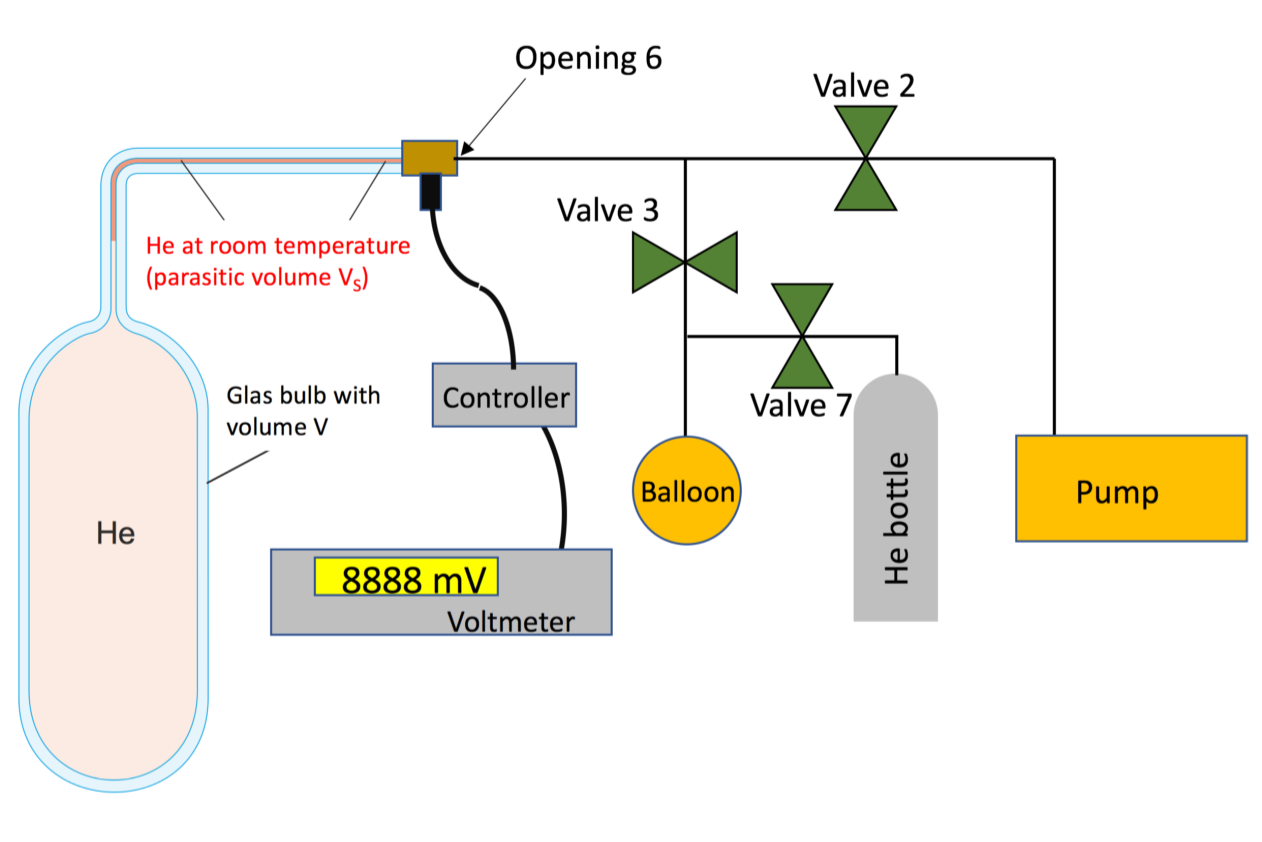
\includegraphics[]{src/images/experimental_setup.png}
        \caption{experimental setup: A glass bulb filled with helium is connected to a sensor and a system of tubes, in turn connecting to a pump, a helium bottle and a baloon.
        The sensor outputs a voltage linearly related to the applied pressure, the pump can reduce the pressure in the bulb, the helium bottle is the helium supply and the balloon acts as a pressure regulator between the bulb and the bottle.
        Multiple valves control the gas flow within the tubes.}
        \label{fig_setup}
    \end{figure}

    Starting with the calibration of the voltmeter, the voltages at room pressure and when a vacuum pump is connected are noted and compared to the actual pressure in the room and the pressure, the pump is able to maintain.
    Hereafter, the glass bulb is evacuated and filled with helium, the reason being that the properties of helium are closer to ideal gases than air.
    Moreover, the oxygen from the air would liquefy when cooled down to the temperature of liquid nitrogen (which would happen in the third step of the experiment series) and liquids do not act according to the ideal gas equation.

    In the next step, the helium-filled glass bulb is heated to the boiling point of water using steam while leaving the apparatus open so that excess helium can escape.
    We chose the temperature of boiling water as the value can easily be calculated using ambient temperature and pressure as well as tabulated data.
    The gas will only expand in this step and hence no air will get into the glass bulb.
    As soon as the helium has reached the desired temperature, the voltage is taken and the system is closed back up at opening 6. (see Fig.~\ref{fig_setup})
    From now on, the closed system can be used just like a thermometer when calculating the temperature at its corresponding voltage.
    
    To create a linear relation of pressure and temperature in the bulb, a second measurement is needed.
    The temperature at the freezing point of water is also known, so this is the second point used in our case.
    The Helium filled bulb is cooled in an ice bath and the voltage is taken.
    To calculate the absolute zero point of temperature, we have to pay respect to the expansion of the glass bulb with increasing temperature.
    Please refer to section~\ref{sec_results} for the calculation.

    As mentioned before, the closed system acts like a thermometer.
    Therefore, we can cool down the helium filled bulb using liquid nitrogen, read off the voltage and calculate the corresponding temperature of liquid nitrogen.
    In this step, the expansion of the glass bulb must be taken into account as well.

    The error sources in this experiment can be classified:
    \begin{itemize}
        \item In our analysis, it is assumed that the temperature in the room stays the same during the whole process.
        Needless to say that this does not have to be the case: small fluctuations happen naturally.
        As a result, corrupted data could occur during the calibration of the sensor.
        Furthermore, the temperature was read off an analog thermometer leading to an uncertainty caused by the limits of the human eye.
        \item Next to the temperature, the pressure does also fluctuate over time.
        The boiling point of water depends on the pressure.
        Hence, when heating the helium to the boiling point of water, a deviation in the temperature used in calculations below and the real temperature could exist.
        As with temperature, the pressure was also read off an analog measurement device and this value could slightly differ from the real pressure.
        \item The manufacturer of the sensor has defined a certain nonlinearity in the conversion of pressure to its corresponding voltage.
        \item The pump does not create an absolute vacuum and small amounts of air could stay in the glass bulb.
        This would have the biggest impact on the temperature measurement of liquid nitrogen as parts of the air would liquify and the linearity resulting from the ideal gas law eq.~\ref{eq_igl} would not be maintained.
        \item When heating and cooling the gas in the bulb, the glass itself could need more time to evenly distribute the temperature resulting in an uneven change in the gas volume, therefore changing the pressure.
        This would affect the difference between the linear approach and the exact calculation of $t_0$ and $t_{LN2}$.
    \end{itemize}


\newpage

\section{Results}\label{sec_results}

    In the first step of this experiment, the pressure sensor has to be calibrated at known pressures and temperatures.
    The result of this calibration is presented in Fig.~\ref{fig_calibration}

    \begin{figure}[H]
        \centering
        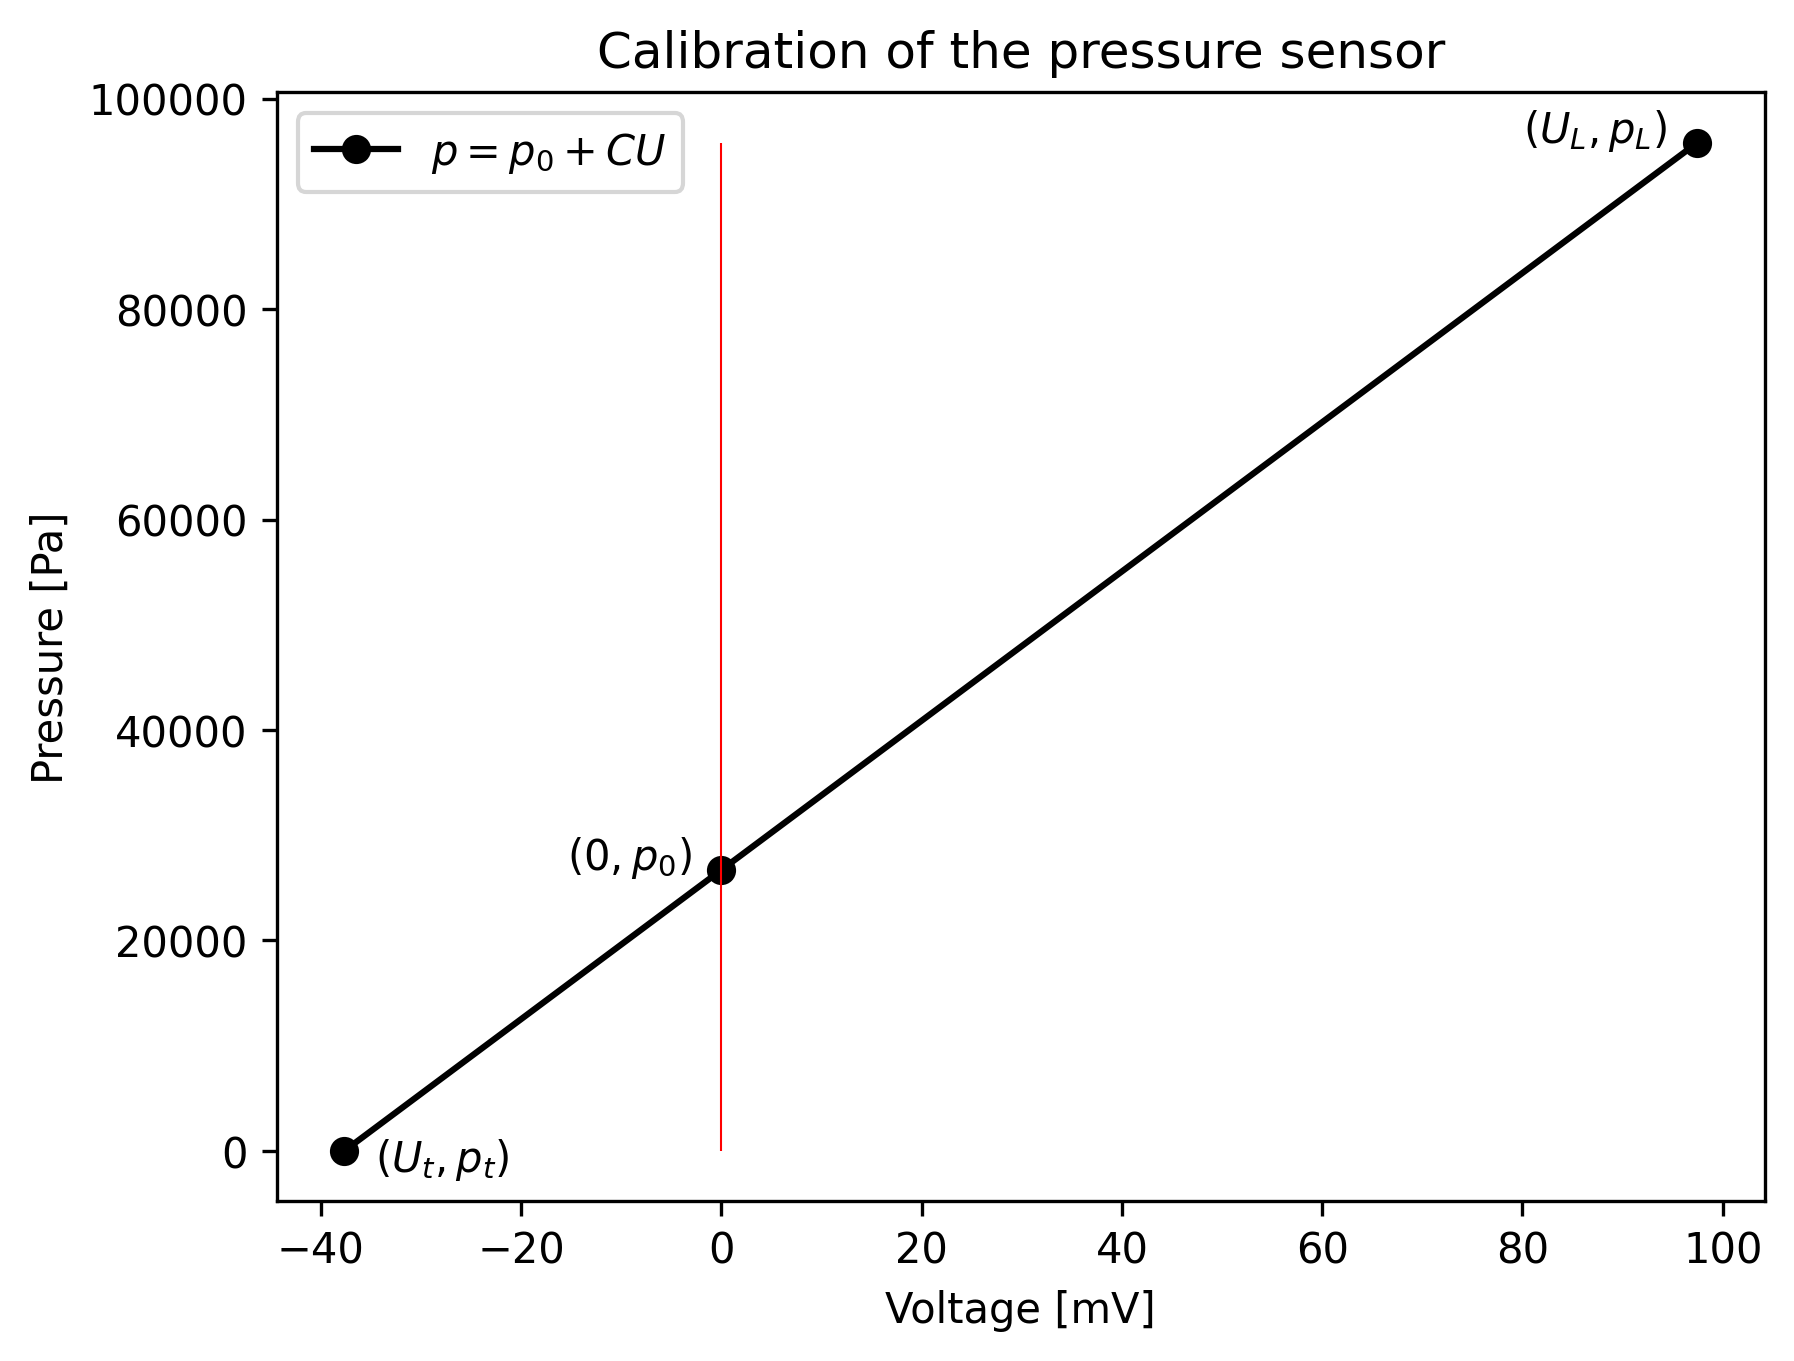
\includegraphics[]{src/images/calibration.png}
        \caption{Calibration of the pressure sensor: A linear fit through $(U_L,p_L)$ and $(U_t,p_t)$ determines the slope $C$. $p_0$ shows the y-intersect at voltage $U_0 = 0$}
        \label{fig_calibration}
    \end{figure}

    Eq.~\ref{eq_c} is used to calculate the slope of this curve. $p_0$ can then be found by entering a pair of known values into eq.~\ref{eq_p0}, such as $(U_t,p_t)$.
    \begin{align}
        C &= \frac{p_L - p_t}{U_L - U_t} \label{eq_c}\\
        p_0 &= p_t - C U_t \label{eq_p0}
    \end{align}

    Using the slope $C$ and y-offset $p_0$, which we determined in this first step, we can calculate the pressure
    of any sensor reading using formula \ref{eq_pressure}.

    \begin{align}
        p(U) = p_0 + CU \label{eq_pressure}
    \end{align}

    To determine the uncertainties in eq.~\ref{eq_pressure}, we first have to calculate the errors in $p_0$, $C$ and $U$.
    Using the gaussian error propagation, we can then determine the error of the entire equation.


    From the manufacturer's datasheet, we know that the linearity of the sensor is guaranteed up to $\pm 0.05\%$ full scale. % of the full scale?
    This means that the sensor signal error is at most $0.05\%$ of $150\si{\milli\volt}$, thus $0.075\si{\milli\volt}$.
    \begin{align}
        \bf \Delta U &= \bf \pm 0.08 ~\si{\bf\milli\volt} \label{dlta_u}
    \end{align}

    Please refer to our jupyter notebook \cite{GitHub}, for the full calculations of all the values and error propagations presented in this chapter.   %LINK GITHUB !!!!

    $\Delta C$ can be determined in a similar way, based on eq.~\ref{eq_c}:
    \begin{align}
        \Delta C &= \sqrt{ \left(\frac{\partial C}{\partial p_L} \Delta p_L \right)^2 +
                        \left(\frac{\partial C}{\partial p_t} \Delta p_t \right)^2 +
                        \left(\frac{\partial C}{\partial U_L} \Delta U_L \right)^2 +
                        \left(\frac{\partial C}{\partial U_t} \Delta U_t \right)^2 } \label{eq_dlta_c}
    \end{align}

    Using the errors for $U$ determined in eq. \ref{dlta_u}, as well as $\Delta p_t = \pm 0.1 \si{\milli\bar}$ given in the manual and $\Delta p_L = 200~\si{\pascal}$,
    we can determine a value for $\Delta C$ using eq.~\ref{eq_dlta_c}:
    \begin{align}
        \Delta C &= \pm 1.878 \label{dlta_c}\\
        \bf C &= \bf 709 \pm 2 ~\si{\bf\pascal/\bf\volt}
    \end{align}

    Lastly, we have to determine the error for $\Delta p_0$. The error can be calculated in the same way as before, based on equation \ref{eq_p0}.
    Due to the fact that the calculated sensor error $\Delta U$ is full scale, it can be assumed for all sensor readings $U_i$.
    \begin{align}
        \Delta p_0 &= \sqrt{ \left(\frac{\partial p_0}{\partial C} \Delta C \right)^2 +
                            \left(\frac{\partial p_0}{\partial U_t} \Delta U_t \right)^2 +
                            \Delta p_t^2}\\
        \Delta p_0 &= \pm 81 ~\si{\pascal} \label{dlta_p0}\\
        \bf p_0 &= \bf (26.7 \pm 0.1) ~\si{\bf\kilo\pascal}
    \end{align}

    We now have all the values for calculating $\Delta p(U)$. Based on eq. \ref{eq_pressure} we can determine the following error propagation:
    \begin{align}
        \Delta p(U) &= \sqrt{ \left(\frac{\partial p}{\partial C} \Delta C \right)^2 +
                            \left(\frac{\partial p}{\partial U} \Delta U \right)^2 +
                            \Delta p_0^2}\\
        &= \sqrt{ \left( U \Delta C \right)^2 +
                \left( C \Delta U \right)^2 + 
                \Delta p_0^2} \label{eq_dlta_p}
    \end{align}

    \begin{figure}[H]
        \centering
        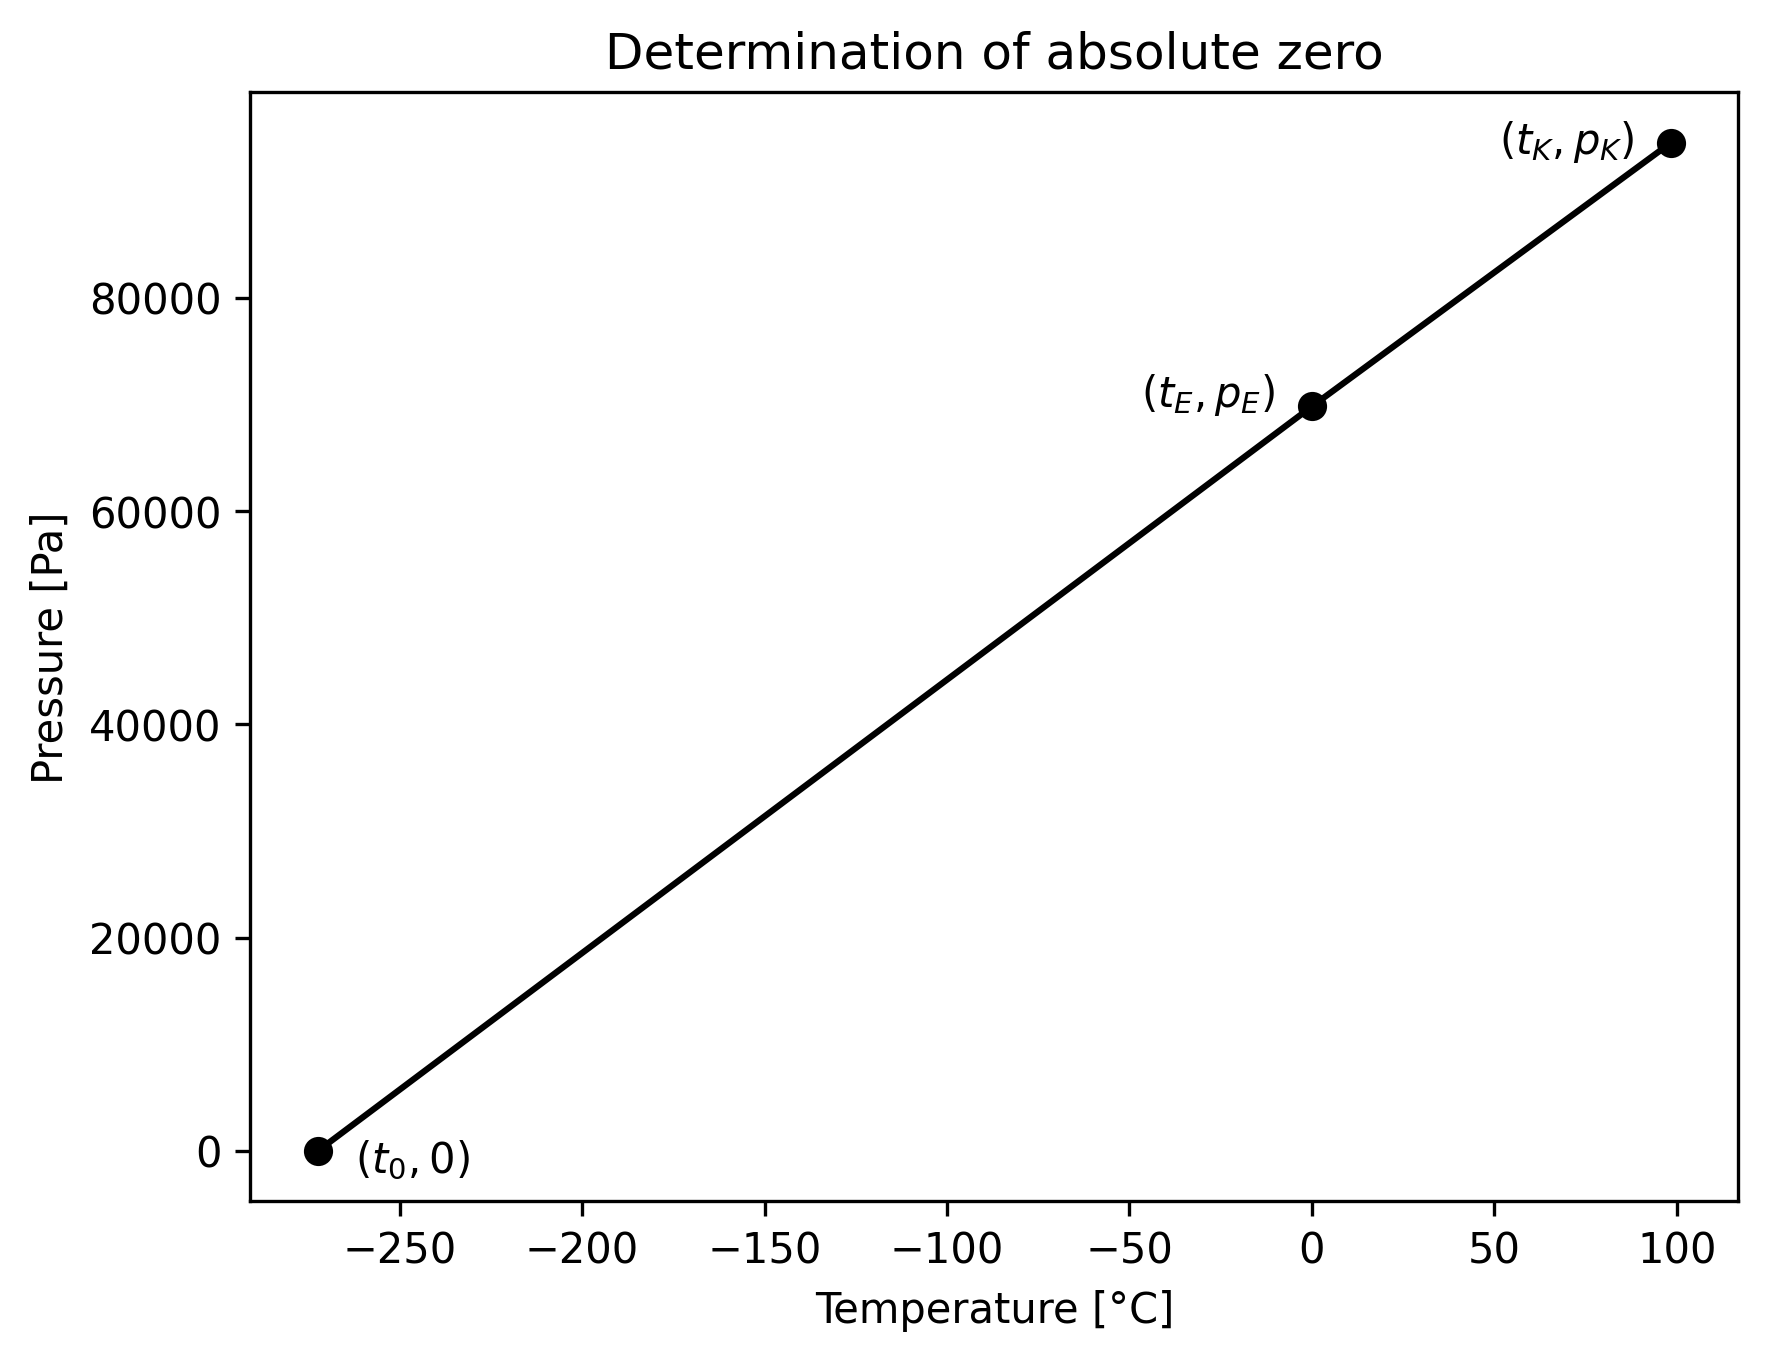
\includegraphics[]{src/images/absolute_zero.png}
        \caption{Determination of absolute zero: Linear fit through $(t_E, p_E)$ and $(t_K, p_K)$ until $p = 0$ is reached.}
        \label{fig_abs_zero}
    \end{figure}
    Fig.~\ref{fig_abs_zero} is a visual representation of how the value for $t_0$ was obtained. Measuring the pressure of the Helium gas at two precisely
    defined temperatures will give us two points on a temperature/pressure graph. The y-intersection of the linear fit through these points will give us an approximative value for $t_0$.
    To get a more precise value, we have to take into account multiple factors like the expansion of the glass bulb under temperature changes, 
    as well as the influence of unevenly heated gas in the connecting tube between the bulb and the sensor.

    In this following paragraph the results from the determination of absolute zero are presented.
    Using eq.~\ref{eq_pressure} the resulting pressures were calculated from the raw sensor data.
    With the derived eq.~\ref{eq_dlta_p} we can then calculate the errors $\Delta p_K, \Delta p_E$. %With the equation derived in eqref...?
    \begin{align}
        p(U_E) &= (69.8 \pm 0.1) ~\si{\kilo\pascal} \label{val_pE}\\
        p(U_K) &= (94.5 \pm 0.2) ~\si{\kilo\pascal} \label{val_pK}
    \end{align}

    As described above the exact value for $t_0$ has to take into account the remaining gas
    in the tube connecting the bulb with the sensor, as well as the thermal expansion of the
    bulb itself. The following quadratic equation calculates the final value for $t_0$ while
    taking into account the factors stated above.
    \begin{align}
        a &= (1 + \varepsilon)p_E - (1 + \epsilon + \gamma t_K)p_K\\
        b &= \varepsilon(p_K - p_E)t_K + (1 + \gamma t_K)p_K t_L - p_E(t_L + t_K)\\
        c &= p_E t_L t_K\\
        t_0 &= \frac{-b \pm \sqrt{b^2 - 4a c}}{2a} \label{eq_t0}
    \end{align}

    Using a barometer in the lab we determined the boiling point of water to be $t_K = 98.323 \si{\celsius}$.
    The temperature in the lab was $t_L = 24 \si{\celsius}$.
    When entering the results from eq.~\ref{val_pE} and~\ref{val_pK}, as well as $t_K$ and $t_L$ into eq.~\ref{eq_t0},
    we get the following result for $t_0$:
    \begin{align}
        t_0 = -275.9~\si{\celsius} \label{val_t0}
    \end{align}

    The error calculation for $t_0$ was again accomplished using the gaussian error propagation.
    Due to the fact that $t_E$, as well as $t_K$, could be determined very precisely, we did not take
    the uncertainties of these values into account in the following error calculation.
    Therefore the only variables whose error margins were considered are $p_E$, as well as $p_K$. % ... whose error margins were considered are...
    \begin{align}
        \Delta t_0 &= \sqrt{ \left(\frac{\partial t_0}{\partial p_E} \Delta p_E \right)^2 +
                            \left(\frac{\partial t_0}{\partial p_K} \Delta p_K \right)^2 }\\
        \Delta t_0 &= \pm 2.45~\si{\celsius} \label{dlta_t0}\\
        \bf t_0 &= \bf (-275.9 \pm 2.45)~\si{\bf\celsius} \label{res_t0}
    \end{align}

    In the last part of the experiment, the apparatus was used as a thermometer, to determine the 
    temperature of liquid nitrogen.
    Using eq.~\ref{eq_pressure} the pressure $p_N$ was calculated from the raw sensor data $U_N$.
    \begin{align}
        p_N = 19.6~\si{\kilo\pascal}
    \end{align}

    To calculate the temperature of liquid nitrogen we can use our known value of $t_0$ and solve
    the following equation for $t'_{LN2}$. This will only give us an approximate value, by simply solving a linear approach.
    \begin{align}
        \frac{p_E}{t_E - t_0} \approx& \; \frac{p_N}{t'_{LN2} - t_0}\\
        t'_{LN2} \approx& \; \frac{p_N}{p_E}(t_E - t_0) + t_0
    \end{align}

    Here we again have to take the volume of gas in the tube connecting the bulb with sensor,
    as well as the shrinkage of the glass bulb due to the temperature change into account.
    The following equation will give us an exact value for $t_{LN2}$:
    \begin{align}
        A \equiv& \; \frac{p_E}{t_E - t_0} + \frac{\varepsilon(p_E - p_N)}{t_L - t_0}\\
        =& \; 253.14~\si{\pascal/\celsius}\\
        t_{LN2} =& \; \frac{A t_0 + p_N}{A - \gamma p_N}\\
        =& \; -198.5~\si{\celsius} \label{val_tN}
    \end{align}

    Using the gaussian error propagation the uncertainty for $t_{LN2}$ was calculated. As stated above
    the uncertainties for the variables $t_L$ and $t_E$ are not considered in this calculation either.
    \begin{align}
        \Delta A =& \; \sqrt{ \left(\frac{\partial A}{\partial p_E} \Delta p_E \right)^2 +
                            \left(\frac{\partial A}{\partial p_N} \Delta p_N \right)^2 +
                            \left(\frac{\partial A}{\partial t_0} \Delta t_0 \right)^2 }\\
        =& \; 2.30~\si{\pascal/\celsius}\\
        \Delta t_{LN2} =& \; \sqrt{ \left(\frac{\partial t_{LN2}}{\partial A} \Delta A \right)^2 +
                                    \left(\frac{\partial t_{LN2}}{\partial t_0} \Delta t_0 \right)^2 +
                                    \left(\frac{\partial t_{LN2}}{\partial p_N} \Delta p_N \right)^2 }\\
        =& \; 2.56~\si{\celsius}\\
        \bf t_{LN2} =& \; \bf (-198.5 \pm 2.56) ~\si{\bf\celsius} \label{res_tN}
    \end{align}

\section{Discussion}
    We have determined the absolute zero temperature to be $t_0 = (-275.9 \pm 2.45)\si{\bf\celsius}$.
    The literature value of $t_{0, \text{lit}} = -273.15 \si{\celsius}$, found on the website britannica \cite{literature_absolute_zero} is within our error margins.
    To depict one major use of the calculated value, it is possible to determine a scientific temperature scale known as the Kelvin scale.
    It takes the absolute zero temperature as the starting point while maintaining the same step between every value as the Celsius scale, so $0 \si{\kelvin} = -273.15 \si{\celsius}$.
    This leads to $1K = \frac{\Delta_{0, E}(T)}{273.16000\cdots}$ with $\Delta_{0, E}(T)$ being the difference in temperature between the absolute zero and the freezing point of water.
    The derived scale is used in domains like thermodynamics.

    We made use of our value for $t_0$ by determining the temperature of liquid nitrogen and obtained a value of $t_{LN2} = (-198.5 \pm 2.56)\si{\bf\celsius}$.
    The literature value of $t_{LN2, \text{lit}} = -195.8 \si{\celsius}$ found on britannica \cite{literature_liquid_nitrogen}.
    Knowing the temperature of liquid nitrogen can be useful when in need of a coolant for future research.

    When comparing each obtained value with the literature values, one can be satisfied with the results the experimental setup delivers.

    Still, the error margin could be reduced.
    The biggest impact is given by the error of the slope from the linear relation, resulting from uncertainties in pressure and temperature.
    One portion of the uncertainty in pressure is due to the sensor.
    A higher precision sensor would reduce the error of the slope $\Delta C$.
    Moreover, the temperature change could affect the reading of the sensor, as it is close to the bulb.
    On the other hand, the further away the sensor is located from the helium bulb, the longer the glass tube connecting both.
    Within this tube, a portion of the Helium receives a different heat than the bulb leading to unevenly heated gas in the apparatus.
    That means the pressure in our system is not exactly proportional to the applied temperature.
    Also, the steam used to heat the bulb to the boiling point of water cools down on its way from the bottom to the top of the bulb, resulting in an uneven change of volume of the glassware.
    Therefore, the volume the gas takes up does not exactly match the calculated value.

    % So far you have discussed how you have obtained your data and the
    % quantities you derived from it. In this , you should discuss
    % the results in the context of physical laws. Depending on the
    % experiment you want to compare your result and its uncertainty with
    % the literature value. If you want to confirm a physical model that
    % explains a certain phenomenon you want to assess if this model
    % describes the data well within the confidence intervals, or whether
    % a simpler model describes the data just as well.


    
    
   

\newpage

\section{Conclusion}
    In this experiment series, we determined the absolute zero temperature $t_0 = (-275.9 \pm 2.45)\si{\bf\celsius}$.
    After having calibrated the apparatus, it could be used as a thermometer and the temperature of liquid nitrogen $t_{LN2} = (-198.5 \pm 2.56)\si{\bf\celsius}$ was found.
    The obtained values are close to the literature values, which confirms the experimental setup to be an effective tool to determine $t_0$ and to use as a thermometer.
    It is possible to derive the Kelvin scale, which serves in different scientific domains, from the values measured and calculated in this experiment.
    However, there are ways to reduce the error margin:
    Waiting for the gas in the apparatus as well as the glass bulb to heat up or cool down is essential to getting the correct result.
    At the same time, the longer we wait, the more air could flow through tiny leaks in the connectons of the tubes.
    Better sealing of the apparatus would ensure less air flow, enable more time for the equilibrium to settle and in turn deliver a better precision of the results.
    Furthermore, monitoring the temperature and pressure of the lab close to the glass bulb while taking the measurement would result in higher certainty.
    Also, a material changing its form less than glass would bring the linear plot closer to the real values

    % In the concluding paragraph you summarize the result, with the
    % emphasis on what you have discovered in this work. You can end this
    % with an outlook on future research, i.e. how could the results be
    % improved or what would be a logical follow up experiment.

\section{Appendix}
    
    \begin{align}
        \text{Ideal gas law: } pV = \nu RT \label{eq_igl}
    \end{align}


\begin{thebibliography}{99}

\bibitem{literature_absolute_zero}
Encyclop\ae dia Britannica, The Editors of Encyclopaedia Britannica, Adam Augustyn, absolute zero, \href{https://www.britannica.com/science/absolute-zero}{website} (last visited: 2023.04.02)

\bibitem{literature_liquid_nitrogen}
Encyclop\ae dia Britannica, R. Thomas Sanderson, Comparison of nitrogen group elements, \href{https://www.britannica.com/science/nitrogen-group-element/Comparison-of-nitrogen-group-elements}{website} (last visited: 2023.04.02)

\bibitem{Manual}
Manual to experiment 9 Absolute Zero (2022).

\bibitem{GitHub}
GitHub Repository containing the Jupyter Notebook we created to calculate all the presented values in this paper. \href{https://github.com/Noothless/Physik-Absolute-Zero}{website}

\end{thebibliography}

\end{document}